\documentclass[sidebar-width=2.25in, primary=slate]{clean-resume} 
\renewcommand{\familydefault}{\sfdefault}

\begin{document}
  \begin{sidebar}
    \avatar[
      scale=3.5,
      yshift=-0.5 cm,
      xshift=-0.25cm,
      size=2cm
    ]{images/selfie.png}
    
    \title{Anish Goyal}[Aspiring Computer Engineer]
    
    \header{Contact}
    
    \contact
    {
      email={anishgoyal1108@gmail.com},
      phone=(470) 451-1404,
      address={Lawrenceville, GA, 30044},
    }
    
    \header{Career Objective}
    
    I am deeply passionate about programming with applications and driven to elevate my skillset. With an unwavering enthusiasm for learning, I am prepared to immerse myself in any given task and collaborate with esteemed mentors and peers to unleash my full potential. I am determined to explore the intricacies of hardware and software, and leverage my knowledge to design innovative solutions and advance technological frontiers. I am confident that I can leverage their cutting-edge resources and guidance to embark on a transformative journey of growth, knowledge acquisition, and meaningful contributions to the field of computer engineering. 
  \end{sidebar}%
  \sep%
  \begin{main}
    \header{Education}
    
    \education
    {
      school = {The Gwinnett School of Math, Science and Technology},
      graduation = {\date{2024/5}},
      gpa = 3.6,
      nga = 90.20
    }
  
    \begin{lst}
      [
        title = {Relevant Coursework},
        columns = 2,
    	]
      \item AP Computer Science Principles (5/5)
      \item AP Computer Science A (5/5)
      \item AP US History (5/5)
      \item AP Comparative Government \& Politics (4/5)
      \item AP US Government \& Politics (3/5)
      \item Data Science \& Analytics II (96/100)
      \item Applications of Linear Algebra in Computer Programming (104/100)
      \item Advanced Calculus II (100/100)
      \item AP Calculus AB (5/5)
      \item AP Biology (4/5)
      \item Engineering Applications (92/100)
      \item Physics \& Engineering (94/100)
      \item CIST 1001: Computer Concepts (95/100)
      \item CIST 1122: Hardware Installation and Maintenance (95/100)
    \end{lst}
    
    \begin{lst}
      [
        title = Clubs,
        columns = 2,
  	]
      \item Computer Science Club
      \item Technology Student Association
      \item Robotics Club
      \item Computer Science Honor Society
    \end{lst}
    
    \header{Experience}
    
    \begin{experience}
      {
        duration = { \range{2023/6} },
        organization = { Schonken and Associates },
        title = { Technical Assistant }
      }
      \item Created cmdlets to automate client onboarding into a Firebase database
    \end{experience}
    
    \begin{experience}
      {
        duration = { \range{2020/9} },
        title = { First Tech Challenge Robotics },
        organization = { 16796 Red Robodragons }
      }
      \item Applied SCRUM, SWOT, and other agile management principles to maintain progress
      \item Created an object-oriented interface with GPIO programming in the REV Robotics Expansion Hub to automate drivetrain movement
    \end{experience}

    \begin{experience}
      {
        duration = { \range{2020/8} },
        title = { Chief of Competitions },
        organization = { GSMST Computer Science Club }
      }
      \item Created weekly seminars in cybersecurity (e.g. rootkit hunting, XSS)
      \item Tutored CS-enrolled students in Python/Java
    \end{experience}

    \begin{experience}
      {
        duration = { \range{2019/10} },
        title = { Sound Engineer },
        organization = { One Mission Church }
      }
      \item Organized the stage and instruments for performers on Sundays
      \item Arranged the band during rehearsals to ensure a good fusion of sound for each service
    \end{experience}

    \header{Proficiencies \& Skills}
    \begin{lst}
      \item \emph{Languages:} R, Python, Java, HTML, CSS, Javascript, PHP, SQL, Bash, Powershell, Perl, Rust, \LaTeX, and C\#
      \item \emph{Libraries:} TensorFlow, Keras, NumPy, Sci-kit Learn, PyTorch, Pandas, OpenCV, Seaborn, Sympy, Matplotlib, Flask, Django, and Bootstrap
      \item \emph{Cloud/DBMS:} MongoDB, AWS, Firebase, VMWare vSphere, and Azure
      \item Proficient in Office 365, Google Workspace, and Adobe Creative Cloud
      \item Introductory fluency in Spanish
    \end{lst}
  \end{main}
  \newpage
  %\begin{sidebar}
    %\hspace*{0.6cm}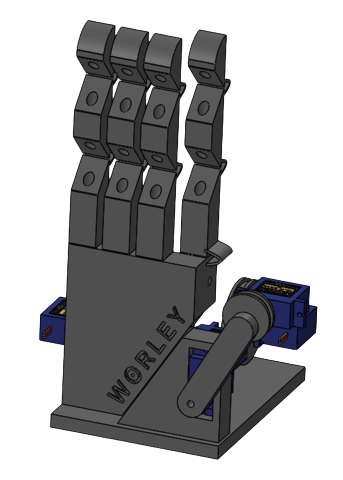
\includegraphics[scale=0.3]{images/hand.png}
    %\hspace*{1.05cm}\vspace*{0.4cm}
\includegraphics[scale=0.07]{images/vim.png}
    %\vspace*{0.3cm}\hspace*{1.05cm}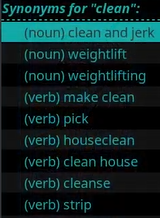
\includegraphics[scale=0.8]{images/rasptd.png}
    %\hspace*{1.05cm}
\includegraphics[scale=0.3]{images/leetcode.png}
    %\hspace*{-0.4cm}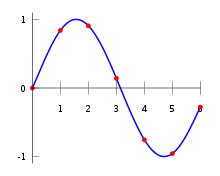
\includegraphics[scale=0.65]{images/polynomial interpolation.png}
    %\hspace*{0.15cm}
\includegraphics[scale=0.40]{images/trophy.png}
  %\end{sidebar}%
  %\sep
    \header{Projects \& Research}

    \begin{experience}
      {
        duration = { \range{2023/6 } },
        title = {A robot hand that can perform sign language in real time},
        organization = {\href{https://github.com/Yubo-Cao/worley}{Wireless Online Real-time Language Expression Yielder (WORLEY)\phantom{aaaaaaaaaaaa}}}
      }
      \item Created a mobile application for live speech input with \verb|WebRTC| audio streaming
      \item Implemented a voice activation detection model on the server to detect speech and extract continuous segments
      \item Integrated OpenAI's \verb|WSPSR| to transcribe speech segments into text
      \item Developed a custom-built transformer model from the \verb|ASLG-PC12| dataset to translate transcribed text to American Sign Language gloss
    \end{experience}

    \begin{experience}
      {
        duration = { \range{2022/10--2022/11 } },
        title = { Vim kanban board editor },
        organization = { \href{https://github.com/anishgoyal1108/VamBan}{VamBan} }
      }
      \item Compiled the program with g++/gcc, linking against the \verb|ncurses| library.
      \item Added support for a variety of terminal sizes, colorschemes, and \verb|i3wm|
    \end{experience}

    \begin{experience}
      {
        duration = { \range{2022/9--2023/5 } },
        title = { Deep learning computer vision model },
        organization = {\href{https://github.com/FIRST-Tech-Challenge/FtcRobotController}{First Tech Challenge Robotics} }
      }
      \item Peformed classification with receptive fields while employing weight decay, alternative learning rate, and transfer learning with a Non-
      Maximum Suppression post-processing layer
      \item Used a single shot multibox detector with ResNet18 as the backbone with 600 labeled images
      \item Exported the model to the ONNX runtime and converted it to a Tensorflow Lite model for deployment
      \item Implemented multi-threading to perform operations in parallel and stored model inferences in a queue for faster response times
    \end{experience}

    \begin{experience}
      {
        duration = { \range{2022/9--2022/10} },
        title = { GUI to help me with trivial English tasks },
        organization = { \href{https://github.com/anishgoyal1108/RASPTD}{Rofi Abbreviator, Speller, Pronouncer, Thesaurus, and Dictionary (RASPTD)} }
      }
      \item Designed a user-friendly GUI for efficient interaction with basic English tools.
      \item Configured all dependencies, including \verb|xclip| for copying selected spelling suggestions to the clipboard, \verb|libnotify| for notifications when copying a spelling suggestion, \verb|tre| for searching a wordlist and providing spelling suggestions, and \verb|sox| for playing pronunciations.
    \end{experience}
    
    \begin{experience}
      {
        duration = { \range{2022/8} },
        title = { A repository with solutions to algorithmic programming problems },
        organization = { \href{https://github.com/Yubo-Cao/algorithms}{Algorithms} }
      }
      \item Tackled challenges in data structures, sorting algorithms, dynamic programming, graph algorithms, mathematical computations, and string manipulation
      \item Participated in competitive programming competitions in school and onlin
    \end{experience}

    \begin{experience}
      {
        duration = { \range{2021/8--2022/5} },
        title = { Science/Engineering fair },
        organization = { \href{https://github.com/anishgoyal1108/Polynomial-Interpolation-and-K-Means-Crime-Prediction-Project}{Polynomial Interpolation and K-Mean Mining to Predict Crime Rates\phantom{aaaaaaaaaaaa}} }
      }
      \item Created a research plan to apply the scientific method and authored a 116-page logbook to communicate my project results
      \item Applied six \verb|sci-kit learn| machine learning algorithms with and without principal component analysis to predict crime rates in Atlanta based on date/time/location
    \end{experience}

    \header{Awards \& Honors}
    
    \begin{lst}
      \item Governor's Honors 
      Program 60 Alumni in Engineering: Computer Programming
      \item Member of the National Society of High School Scholars
      \item Member of the Computer Science Honor Society
      \item AP Scholar With  Distinction
      \item USACO silver medalist
      \item CyberPatriot national semifinalist
      \item 3rd place nationally in Lockheed Martin's CodeQuest 2023
      \item 8th place nationally in picoCTF 2023
      \item Two-time robotics state champions (2021 \& 2022)
      \item Participation in the 2nd annual Georgia Tech Probability \& Statistics Competition
    \end{lst}
\end{document}